\documentclass[12pt]{article}
\usepackage{common}
\usepackage{amsmath}
\usepackage{setspace}
\usepackage{graphicx}
\usepackage{tikz}
\usepackage{subfig}
\usepackage{float}
\tikzset{> = latex, every picture/.style={line width=0.7pt}}

\pdfpagewidth 8.5in
\pdfpageheight 11in 

\setlength\topmargin{0in}
\setlength\headheight{0in}
\setlength\headsep{0in}
\setlength\textheight{9in}
\setlength\textwidth{5.5in}
\setlength\oddsidemargin{.5in}
\setlength\evensidemargin{.5in}
\setlength\parindent{0.25in}
\setlength\parskip{0in}

\newboolean{solutionCopy}
\setboolean{solutionCopy}{true} % Toggle between solution copy and distro

\ifthenelse{\boolean{solutionCopy}}{
  \includeversion{solution}
}{
  \excludeversion{solution}
}

\begin{document}

\singlespacing

\begin{center}
{\Large\textbf{CS 181: Bayesian Networks, HMMs, and Kalman Filters}} \\
\vspace{.5cm}
{\large Week of April 9, 2018 \\
 Harvard University}
\end{center}
\vspace{.5cm}

%\section{Bayesian Networks Continued}
%
%Recall that a Bayesian network is a graphical model that represents random variables and their dependencies using a directed acyclic graph. They allow us to efficiently model joint distributions over many variables by taking advantage of the local dependencies between variables, and they form the foundation of other models that we'll explore today.
%
%\subsection{D-separation rules}
%
%$X_A$ and $X_B$ are \textit{d-separated} by evidence $X_E$ if every undirected path from $X_A$ to $X_B$ is ``blocked'' by $X_E$. A path is blocked by evidence $X_E$ if either:
%
%\begin{enumerate}
%	\item There is a node $Z$ with non-converging arrows on the path, and $Z \in X_E$.
%	\item There is a node $Z$ with ``converging arrows on the path, and neither $Z$ nor its descendants are in $X_E$.
%\end{enumerate}
%\newpage
%
%\section{Reasoning about the Correctness of Networks}
%
%\begin{figure}[htp]
%	\begin{center}
%		\begin{tikzpicture}
%		\begin{scope}[every node/.style={circle,draw,minimum size=2.55em}]
%		\node (F1) at (-1,3) {$F_1$};
%		\node (F2) at (1,3) {$F_2$};
%		\node (M1) at (-1,1.5) {$M_1$};
%		\node (M2) at (1,1.5) {$M_2$};
%		\node (N) at (0,0) {$N$};
%		\end{scope}
%		
%		\begin{scope}[every edge/.style={draw}]
%		\path [->] (F1) edge (M1);
%		\path [->] (F2) edge (M2);
%		\path [->] (M1) edge (N);
%		\path [->] (M2) edge (N);
%		\end{scope}
%		
%		\node at (0,-1) {(i)};
%		\end{tikzpicture} \qquad
%		\begin{tikzpicture}
%		\begin{scope}[every node/.style={circle,draw,minimum size=2.55em}]
%		\node (F1) at (-1.5,0) {$F_1$};
%		\node (F2) at (1.5,0) {$F_2$};
%		\node (M1) at (-1.5,-3) {$M_1$};
%		\node (M2) at (1.5,-3) {$M_2$};
%		\node (N) at (0,0) {$N$};
%		\end{scope}
%		
%		\begin{scope}[every edge/.style={draw}]
%		\path [->] (F1) edge (M1);
%		\path [->] (F2) edge (M2);
%		\path [->] (N) edge (M1);
%		\path [->] (N) edge (M2);
%		\end{scope}
%		
%		\node at (0,-4) {(ii)};
%		\end{tikzpicture} \qquad
%		\begin{tikzpicture}
%		\begin{scope}[every node/.style={circle,draw,minimum size=2.55em}]
%		\node (F1) at (-1.5,-1.5) {$F_1$};
%		\node (F2) at (1.5,-1.5) {$F_2$};
%		\node (M1) at (-1.5,1.5) {$M_1$};
%		\node (M2) at (1.5,1.5) {$M_2$};
%		\node (N) at (0,0) {$N$};
%		\end{scope}
%		
%		\begin{scope}[every edge/.style={draw}]
%		\path [->] (M1) edge (M2);
%		\path [->] (M1) edge (F1);
%		\path [->] (M2) edge (F2);
%		\path [->] (M1) edge (N);
%		\path [->] (M2) edge (N);
%		\path [->] (N) edge (F1);
%		\path [->] (N) edge (F2);
%		\end{scope}
%		\node at (0,-2.5) {(iii)};
%		\end{tikzpicture}
%		
%	\end{center}
%\end{figure}
%
%\fbox{\parbox{\linewidth}{%
%Two astronomers in different parts of the world make measurements
%$M_1$ and $M_2$ of the number of stars $N$ in some small region of the
%sky. Each telescope may be badly out of focus (events $F_1$ and
%$F_2$). Consider the Bayesian networks above.
%
%\begin{enumerate}
%			\item Which of these Bayesian networks correctly represents the distribution? 
%			\item Of the correct networks, why might one be preferred?
%\end{enumerate}
%}}
%\medskip
%\begin{solution}
%\begin{enumerate}
%		\item Network~(i) is incorrect. It states, for example, that $I(N, F_1 \given M_1, M_2)$, whereas we
%		know that $F_1$ still provides information about $N$ conditioned on the two measurements (what if telescope
%		1 is faulty?).
%		\medskip
%		
%		Network~(ii) is correct. Consider ordering $F_1, N, F_2, M_1, M_2$. We
%		can check that $N$ is independent of $F_1$, $F_2$ is independent of
%		$N$ and $F_1$, $M_1$ depends on $F_1$ and $N$ but not $F_2$, and $M_2$
%		depends on $F_2$ and $N$ but not $F_1$, and not $M_1$ when conditioned
%		on $N$.
%		\medskip
%		
%		Network~(iii) is correct. Consider ordering $M_1, M_2, N, F_1, F_2$. The
%		only edges omitted when constructing the network are
%		
%		-- from $M_2$ to $F_1$, but conditioned on $N$ and $M_1$ then $M_2$ provides no
%		information about $F_1$.
%		
%		-- from $M_1$ to $F_2$ (same argument) and from $F_1$ to $F_2$,
%		and $F_1$ provides no information about $F_2$ when conditioned on
%		$N$ and $M_2$.\\
%		
%		\item Network (ii) may be preferable because it represents all of the necessary dependences while using fewer edges and, hence, fewer parameters. That is, network (ii) expresses the distribution more efficiently. 
%\end{enumerate}
%
%\end{solution}

%\ifthenelse{\boolean{solutionCopy}}{}{\vspace{5cm}}

\section{Variable Elimination in Bayesian Networks}
Recall that a Bayesian network is a graphical model that represents random variables and their dependencies using a directed acyclic graph. They allow us to efficiently model joint distributions over many variables by taking advantage of the local dependencies between variables, and they form the foundation of other models that we'll explore today.\\

In this section, we discuss an exact inference algorithm called variable elimination. Consider the Bayesian network we saw in lecture:
% \begin{center}
% 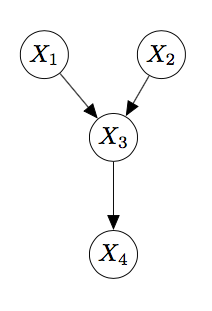
\includegraphics[width=2in]{lecture_network}
% \end{center}

\begin{figure}[htp]
\begin{center}

\begin{tikzpicture}
\begin{scope}[every node/.style={circle,draw,minimum size=2.55em}]
\node (X1) at (-1.5,4.5) {$X_1$};
\node (X2) at (1.5,4.5) {$X_2$};
\node (X3) at (0,2.5) {$X_3$};
\node (X4) at (0,0) {$X_4$};
\end{scope}

\begin{scope}[every edge/.style={draw}]
    \path [->] (X1) edge (X3);
    \path [->] (X2) edge (X3);
    \path [->] (X3) edge (X4);
\end{scope}
\end{tikzpicture}

\end{center}
\end{figure}

Assume that all of the random variables are Bernoulli, meaning their domain is $\{0, 1\}$, and thus the domain size $k = 2$. In this network, we can encode the joint distribution as
\begin{align} p(x_1, x_2, x_3, x_4) = p(x_3 | x_1, x_2)p(x_4 | x_3)p(x_1)p(x_2)\end{align}

If we wanted to calculate the marginal distribution of $X_4$, we could naively marginalize out the other variables, giving us
\begin{align}
p(x_4) = \sum_{x_1}\sum_{x_2}\sum_{x_3}p(x_3 | x_1, x_2)p(x_4 | x_3)p(x_1)p(x_2)
\end{align}
Calculating this naively requires multiplying 4 values for each of the 8 possible combinations of $x_1, x_2, x_3$.
In general, if there were many variables then the number of combinations would grow exponentially
in the number of variables!
%
%$x_1, x_2,x_3$ were not Bernoulli but could take on several different values, the number of terms in the sum would grow very large!
%Thus, for each value of $x_4$, we must multiply 32 terms and then add 8 terms for each value of $x_4$, leading to a total of 80 steps.

However, note that because we have a compact, Bayesian net representation, 
we can  calculate the marginal distribution more efficiently. By reordering the sums and eliminating one variable at a time, we derive the variable elimination procedure. For example, we can calculate the joint distribution as:
\begin{align}
p(x_4) &= \sum_{x_1, x_2, x_3}p(x_3 | x_1, x_2)p(x_4 | x_3)p(x_1)p(x_2) \\
&= \sum_{x_2, x_3}p(x_4 | x_3)p(x_2)\sum_{x_1}p(x_3 | x_1, x_2)p(x_1) \\
&= \sum_{x_3}p(x_4 | x_3)\sum_{x_2}p(x_2)p(x_3 | x_2)\\
&= \sum_{x_3}p(x_4 | x_3)p(x_3)\\
&= p(x_4)
\end{align}

Here, we eliminate $x_1$, then $x_2$, then $x_3$. This is working in
`leaves first' order towards the query, $x_4$.  Alternatively, we
could have eliminated variables in a different order, as follows:

\begin{align}
p(x_4) &= \sum_{x_1, x_2, x_3}p(x_3 | x_1, x_2)p(x_4 | x_3)p(x_1)p(x_2) \\
&= \sum_{x_1, x_2}p(x_1)p(x_2)\sum_{x_3}p(x_3 | x_1, x_2)p(x_4 | x_3) \\
&= \sum_{x_1}p(x_1)\sum_{x_2}p(x_2)p(x_4 | x_1, x_2)\\
&= \sum_{x_1}p(x_1)p(x_4 | x_1)\\
&= p(x_4)
\end{align}

Here, we eliminate $x_3$, then $x_2$, then $x_1$.

\newpage


\fbox{\parbox{\linewidth}{%
\textbf{Variable Elimination.} For the following questions, consider the Bayesian network described above, and assume the following CPTs:
%
\begin{center}
	\begin{tabular}{|c|c|}
		\hline
		{$x_1$}&{$p(x_1)$} \\
		\hline
		0&0.3\\
		1&0.7\\
		\hline
	\end{tabular} \
	\begin{tabular}{|c|c|}
		\hline
		{$x_2$}&{$p(x_2)$} \\
		\hline
		0&0.6\\
		1&0.4\\
		\hline
	\end{tabular} \
	\begin{tabular}{|c|c|c|c|}
		\hline
		{$x_3$}&{$x_1$}&{$x_2$}&{$p(x_3 | x_1, x_2)$} \\
		\hline
		0&0&0&0.5\\
		0&0&1&0.2\\
		0&1&0&0.9\\
		0&1&1&0.5\\
		1&0&0&0.5\\
		1&0&1&0.8\\
		1&1&0&0.1\\
		1&1&1&0.5\\
		\hline
	\end{tabular} \
	\begin{tabular}{|c|c|c|}
		\hline
		{$x_4$}&{$x_3$}&{$p(x_4 | x_3)$} \\
		\hline
		0&0&0.7\\
		0&1&0.1\\
		1&0&0.3\\
		1&1&0.9\\
		\hline
	\end{tabular}
\end{center} 
\medskip 

\begin{enumerate}
	\item First use variable elimination on $X_1$. Draw the resulting Bayesian network and compute the CPT.
	\item First use variable elimination on $X_3$. Draw the resulting Bayesian network and compute the CPT.
\end{enumerate}
How many sum-product calculations do each of these variable elimination orders require? Which one is preferable?
}}

\begin{solution}

\begin{enumerate}
\item The resulting network is:
\begin{center}

\begin{tikzpicture}
\begin{scope}[every node/.style={circle,draw,minimum size=2.55em}]
% \node (X1) at (-1.5,4.5) {$X_1$};
\node (X2) at (0,5) {$X_2$};
\node (X3) at (0,2.5) {$X_3$};
\node (X4) at (0,0) {$X_4$};
\end{scope}

\begin{scope}[every edge/.style={draw}]
    % \path [->] (X1) edge (X3);
    \path [->] (X2) edge (X3);
    \path [->] (X3) edge (X4);
\end{scope}
\end{tikzpicture}
\end{center}

The variable elimination process eliminates $X_1$ by marginalizing out $X_1$: $p(x_3 | x_2) = \sum_{x_1} p(x_3 | x_1, x_2) p(x_1)$. For example: 
\begin{align*}
    p(X_3 = 0 | X_2 = 0) &= \sum_{x_1\in\{0,1\}} p(X_3 = 0 | X_1 = x_1, X_2 = 0) p(X_1 = x_1)\\
    &= 0.5 \cdot 0.3 + 0.9 \cdot 0.7\\
    &= 0.78
\end{align*}

This is a `sum-product calculation'.
We need to do this for each value of $X_2$ and $X_3$. 
Thus, there are four sum-product calculations
to perform. 
The resulting CPT is:\\
%
\begin{center}
\begin{tabular}{|c|c|c|}
\hline
{$x_3$}&{$x_2$}&{$p(x_3 | x_2)$} \\
\hline
0&0&0.78\\
0&1&0.41\\
1&0&0.22\\
1&1&0.59\\
\hline
\end{tabular}
\end{center}
\medskip

\item The resulting network is 
\begin{center}

\begin{tikzpicture}
\begin{scope}[every node/.style={circle,draw,minimum size=2.55em}]
\node (X1) at (-1.5,2.5) {$X_1$};
\node (X2) at (1.5,2.5) {$X_2$};
\node (X4) at (0,0) {$X_4$};
\end{scope}

\begin{scope}[every edge/.style={draw}]
    \path [->] (X1) edge (X4);
    \path [->] (X2) edge (X4);
\end{scope}
\end{tikzpicture}

\end{center}

The variable elimination process eliminates $X_3$ by marginalizing out $X_3$: $p(x_4 | x_1, x_2) = \sum_{x_3} p(x_4 | x_3) p(x_3 \mid x_1, x_2)$. This would be the first intermediate term. 
For example: 
\begin{align*}
    p(X_4 = 0 | X_1 = 0, X_2 = 0) &= \sum_{x_3\in\{0,1\}} p(X_4 = 0 | X_3 = x_3) p(X_3 = x_3 | X_1 = 0, X_2 = 0)\\
    &= 0.7 \cdot 0.5 + 0.1 \cdot 0.5\\
    &= 0.40
\end{align*}

We need to do this for each value of $X_1, X_2$ and $X_4$. Thus,
there are eight sum-product calculations to perform. 
The resulting CPT is:
%
\begin{center}
\begin{tabular}{|c|c|c|c|}
\hline
{$x_4$}&{$x_1$}&{$x_2$}&{$p(x_4 | x_1, x_2)$} \\
\hline
0&0&0&0.40\\
0&0&1&0.22\\
0&1&0&0.64\\
0&1&1&0.40\\
1&0&0&0.60\\
1&0&1&0.78\\
1&1&0&0.36\\
1&1&1&0.60\\
\hline
\end{tabular}
\end{center}
 
\item In these variable elimination operations, we 
%are calculating intermediate distributions in the marginalization for $p(x_4)$. 
%
need to compute intermediate terms. The cost of computing these intermediate terms depends on the
number of variables that they mention, because we have a sum product calculation for each mention.

For the first ordering, the intermediate terms are:
%
\begin{itemize}
\item $p(x_3\given x_2)$: mentions $x_2$ and $x_3$, and thus four sum-product calculations (for each row
in the earlier CPT)
\item $p(x_3)$: mentions $x_3$ and thus two sum-product calculations
\item $p(x_4)$: mentions $x_4$ and thus two sum-product calculations
\end{itemize}

We have a total of $4+2+2=8$ sum-product calculations.

For the second ordering, the intermediate terms are:
%
\begin{itemize}
\item $p(x_4\given x_1,x_2)$: mentions $x_1$, $x_2$ and $x_4$, and thus eight sum-product calculations (for each row
in the earlier CPT).
\item $p(x_4\given x_1)$: mentions $x_1$ and $x_4$,  and thus four sum-product calculations
\item $p(x_4)$: mentions $x_4$ and thus two sum-product calculations
\end{itemize}

We have a total of $8+4+2=14$ sum-product calculations.
%
%In the first ordering, we first calculate $p(x_3 | x_2) = \sum_{x_1}p(x_3 | x_1, x_2)p(x_1)$. This requires adding 4 terms. We then calculate $p(x_3) = \sum_{x_2}p(x_2)p(x_3 | x_2)$, which requires adding 2 terms. Lastly, we calculate $p(x_4) = \sum_{x_3}p(x_4 | x_3)p(x_3)$, which requires adding 2 terms. This is a total of 8 additions.
%
%In the second process, we first calculate
%$p(x_4 | x_1, x_2) = \sum_{x_3}p(x_3 | x_1, x_2)p(x_4 | x_3)$. This has 8 additions. We then calculate $p(x_4 | x_1) = \sum_{x_2}p(x_2)p(x_4 | x_1, x_2)$, which has 4 additions. Lastly, we calculate $p(x_4) = \sum_{x_1}p(x_1)p(x_4 | x_1)$, which has 2 additions. This is a total of 14 additions.

Thus, we see that the first ordering requires fewer computational steps.
\end{enumerate}
\end{solution}

\newpage

\section{Hidden Markov Models}

Last week in lecture, we covered Hidden Markov Models (HMMs). This model is useful for inferring a sequence of unknown states from a corresponding sequence of observed evidence.

%Consider the following two examples:\\
%
%\begin{enumerate}
%	\item Speech Recognition: Your $N$ data points $\{\mathbf{x}^i\}_{i=1}^N$ are recordings of human speech, each segmented into $n$ time steps. Given a sequence of audio information, you would like to infer the true sequence of discrete words that speaker $i$ intended to communicate.\\
%	
%	\item Facial Expression Recognition / Affective Computing: Each data entry is a sequence of photographs of a single person's face over a short period of time. Using these photo sequences as your observations, you would like to infer a sequence of associated underlying emotions/affects/moods that the human was experiencing.\\
%\end{enumerate}
%
%Practical Note: notice that in the first example, we also have the problem of effectively segmenting the observation into time steps, while the second example's observations are already discrete over time.


\subsection{HMM Graphical Model}

\begin{center}
	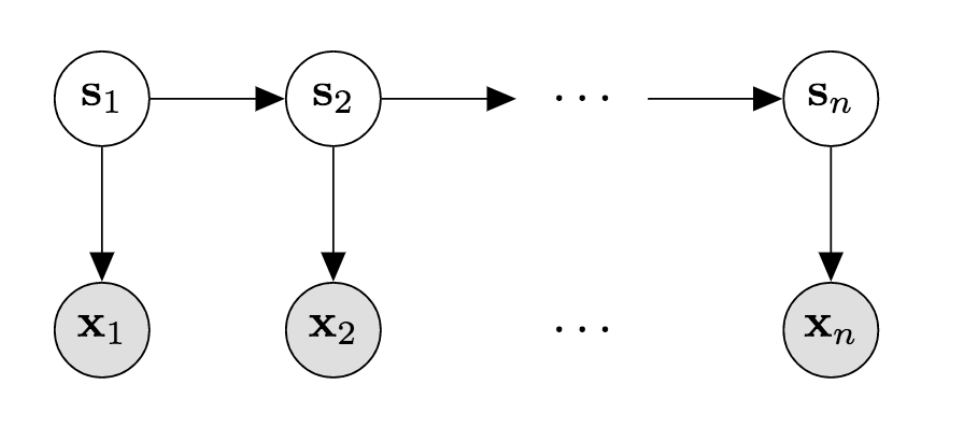
\includegraphics[scale = 0.4]{hmm_generic.jpg}
\end{center}


Consider a sequence of one-hot encoded states $\mathbf{s}_1$,...,$\mathbf{s}_n$ where $\mathbf{s}_t \in \{S_k\}_{k=1}^c$ and a corresponding sequence of observations
$(\mathbf{x}_1$,...,$\mathbf{x}_n)$ where $\mathbf{x}_t \in \{O_j\}_{j=1}^m$. Each state can be one of $c$ possible states, and each observation can be one of $m$ possible observations. Note that $N$ is the number of data points (each of which is a sequence), where $n$ is the length of a sequence (assume all sequences are the same length). HMMs are characterized by, and help us reason about, the following joint distribution:
\begin{align*}
p(\boldsymbol{s}_1,\ldots,\boldsymbol{s}_n,\mathbf{x}_1,\ldots,\mathbf{x}_n) &= \\ 
p(\boldsymbol{s}_1,\ldots,\boldsymbol{s}_n)p(\mathbf{x}_1,\ldots,\mathbf{x}_n\given \boldsymbol{s}_1,\ldots,\boldsymbol{s}_n) &= \\p(\boldsymbol{s}_1)\prod_{t=1}^{n-1}p(\boldsymbol{s}_{t+1}\given \boldsymbol{s}_{t})\prod_{t=1}^n p(\mathbf{x}_t\given\boldsymbol{s}_t)
\end{align*}

Parameters:

\begin{itemize}
	
	\item $\boldsymbol{\theta}$: distribution over initial states, $c \times 1$
	
	\item $\mathbf{T}$: $c \times c$ transition matrix such that $t_{kj}$ is the probability of transitioning from $S_k$ to $S_j$
	
	\item $\{\boldsymbol{\pi}\}_{k=1}^c$: state conditional observation probabilities such that $p(\mathbf{x}_t = O_j | \mathbf{s}_t = S_k; \{\boldsymbol{\pi}\}) = \pi_{kj}$. Each $\boldsymbol{\pi}_k$ is $m \times 1$.
	
\end{itemize}

Our goals are twofold. First, we need to estimate the parameters from the data. We will do this with a special variant of EM. Then, with our trained HMM, we are able to perform several inference tasks on our data, including smoothing, prediction, and more (see below).


\subsection{Properties of HMMs}

\begin{itemize}
	
	\item future is independent of past given present (Markov Property):
	
	$p(\boldsymbol{s}_{t+1}\given \boldsymbol{s}_{1},\ldots\boldsymbol{s}_{t},\mathbf{x}_1,\ldots,
	\mathbf{x}_t)=p(\boldsymbol{s}_{t+1}\given \boldsymbol{s}_t)$
	
	
	
	\item observations only depend on present:
	
	$p(\mathbf{x}_t\given \boldsymbol{s}_1,\ldots,\boldsymbol{s}_t,\mathbf{x}_1,\ldots,\mathbf{x}_{t-1})=
	p(\mathbf{x}_t\given \boldsymbol{s}_t)$
	
\end{itemize}


\subsection{EM for HMMs: finding parameters with the Baum-Welch Algorithm}

Given data points $\{\mathbf{x}^i\}_{i=1}^N$ defined by sequences $(x_1^{i},\ldots,x_n^{i})$ of length $n$ represented as row vectors, we want to infer the parameters $\{\mathbf{T}, \boldsymbol{\theta}, \{\boldsymbol{\pi}_k\}\}.$ Had we been given the true states, we could easily compute joint probability $p(\mathbf{x}^i,\bolds^i)$ and write the complete-data log likelihood, and maximize with respect to the parameters. Instead, we must proceed by estimating state distributions and parameters iteratively.


\subsubsection{Forward-Backward}


The HMM model is characterized by the joint distribution $p(\boldsymbol{s}_1,\ldots,\boldsymbol{s}_n,\mathbf{x}_1,\ldots,\mathbf{x}_n)$, which means that many of our training and inference tasks are an issue of marginalizing to obtain conditionals. Thus, naive algorithms can be expensive (lots of nested summations over states). EM for HMMs using the efficient Forward-Backward inference algorithm is called the Baum-Welch algorithm. Following the algorithm, we define the recurrence relations $\alpha_t(\boldsymbol{s}_t)$ and $\beta_t(\boldsymbol{s}_t)$ in the E step:

\begin{itemize}
	
	\item $\alpha_t(\bolds_t)$ represents the joint probability of observations $1,\ldots,t$ and state $t$. $\alpha_t$ can be defined in terms of $\alpha_{t-1}$. Move \textbf{forwards} through the sequence to calculate the $\alpha$'s
	
	\item $\beta_t(\bolds_t)$ represents the joint probability of observations $t+1,\ldots,n$ conditioned on state $t$. $\beta_{t}$ can be defined in terms of $\beta_{t+1}$. Move \textbf{backwards} through the sequence to calculate the $\beta$'s.
	
\end{itemize}


\begin{figure}[H]%
	\centering
	\subfloat[alpha]{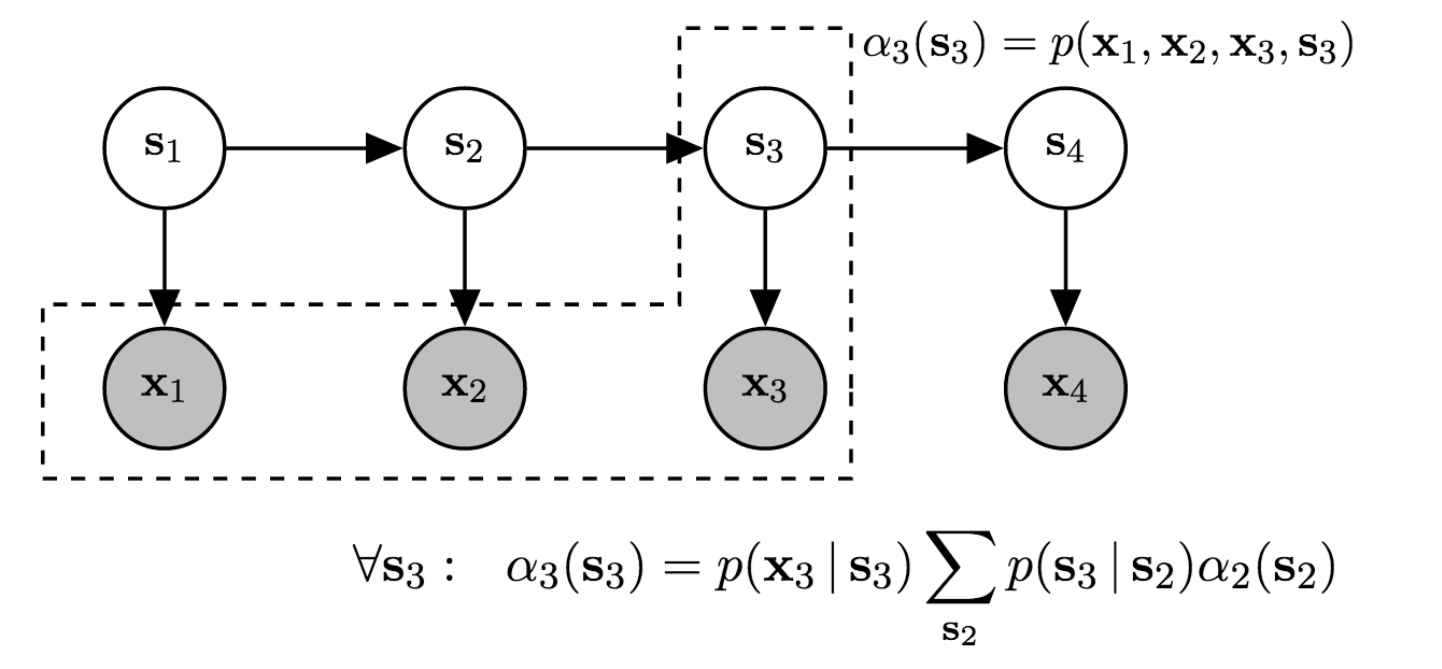
\includegraphics[scale=.15]{alpha.png}}%
	\qquad
	\subfloat[beta]{{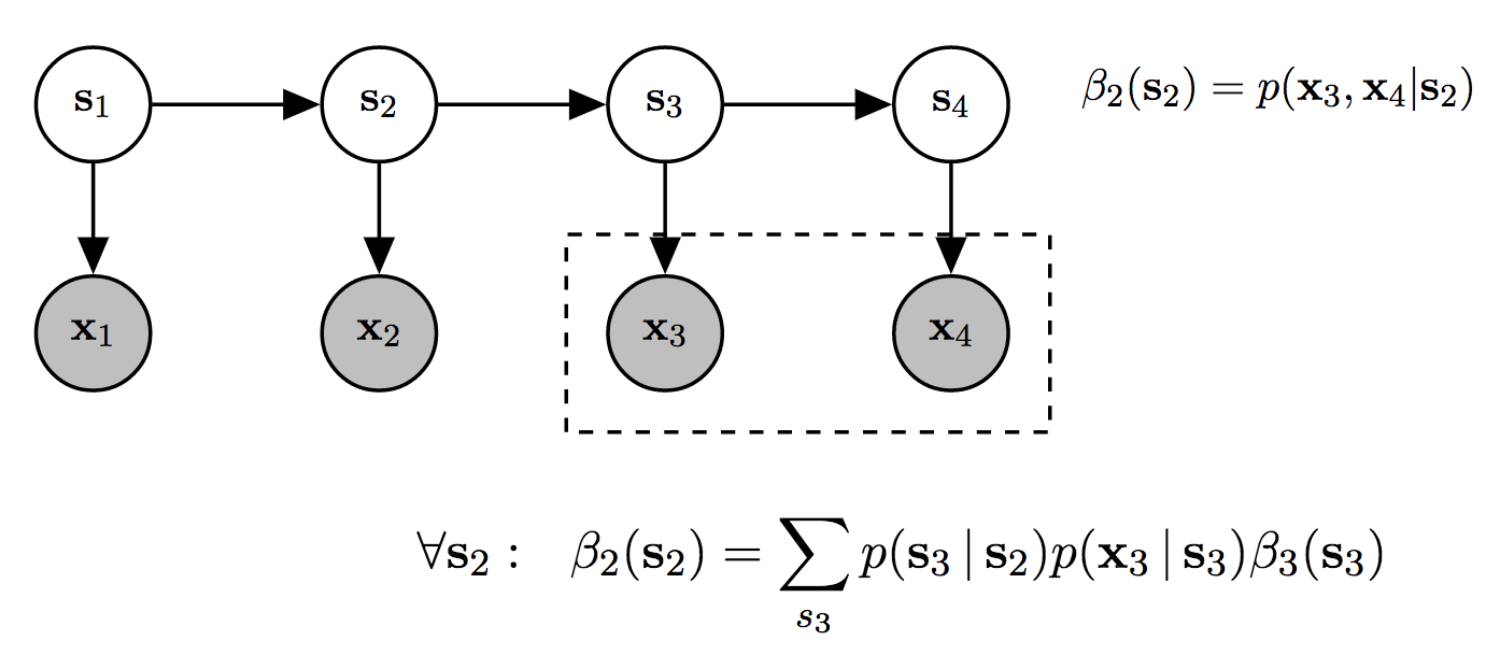
\includegraphics[scale=.15]{beta.png} }}%
	\label{fig:example}%
\end{figure}

The probabilities used in the $\alpha$ and $\beta$ definitions come from the parameters that we fix in the E step.

{\small 
	\begin{align*}
	\forall \bolds_t:\ \ 
	\alpha_t(\bolds_t)&=\left\{
	\begin{array}{ll}
	p(\boldx_t\given \bolds_t)\sum_{\bolds_{t-1}} p(\bolds_t\given\bolds_{t-1})\alpha_{t-1}(\bolds_{t-1}) &\mbox{if $1<t\leq n$}\\
	p(\boldx_1\given \bolds_1)p(\bolds_1) &\mbox{o.w.}
	\end{array}
	\right.
	\end{align*}
}

{\small
	\begin{align*}
	\forall \bolds_t:\ \ 
	\beta_t(\bolds_t)&=\left\{
	\begin{array}{ll}
	\sum_{\bolds_{t+1}} p(\bolds_{t+1}\given\bolds_{t})
	p(\boldx_{t+1}\given\bolds_{t+1})\beta_{t+1}(\bolds_{t+1})
	&\mbox{if $1\leq t< n$}\\
	1 &\mbox{o.w.}
	\end{array}
	\right.
	\end{align*}
}

\subsubsection{Inference Patterns with $\boldsymbol{\alpha},\boldsymbol{\beta}$}

The following patterns are useful for inference with a trained HMM, but also in the E step during training (basically, any time we are considering the parameters fixed):

\begin{itemize}
	
	\item  $\alpha_t(\bolds_t)\beta_t(\bolds_t) = p(\boldx_1,\ldots,\boldx_n,\bolds_t) \propto p(\bolds_t | \boldx_1,\ldots,\boldx_n)$
	
	\item joint of observations: $p(\boldx_1,\ldots,\boldx_n)=\sum_{\bolds_t}\alpha_t(\bolds_t)\beta_t(\bolds_t)$ (for any $t$)
	
	\item smoothing: $p(\bolds_t\given \boldx_1,\ldots,\boldx_n)\propto p(\boldx_1,\ldots,\boldx_n,\bolds_t)=\alpha_t(\bolds_t)\beta_t(\bolds_t)$
	
	\item prediction: $p(\boldx_{n+1}\given \boldx_1,\ldots,\boldx_n)
	\propto\sum_{\bolds_n, \bolds_{n+1}}\alpha_n(\bolds_n)
	p(\bolds_{n+1}\given \bolds_n)
	p(\boldx_{n+1}\given \bolds_{n+1})$
	
	\item transition: $p(\bolds_t,\bolds_{t+1}\given \boldx_1,\ldots,\boldx_n)
	\propto\alpha_t(\bolds_t)p(\bolds_{t+1}\given\bolds_t)p(\boldx_{t+1}\given\bolds_{t+1})\beta_{t+1}(\bolds_{t+1})$
	
\end{itemize}

\subsubsection{E step}

For sequence $\mathbf{x}^i$ and a fixed set of parameters $\boldw = \{\mathbf{T}, \boldsymbol{\theta}, \{\boldsymbol{\pi}_k\}\}$, we estimate the state distribution for $\bolds_1^i,\ldots,\bolds_n^i$ given $\mathbf{x}^i$. Let the $c \times 1$ vector $\boldq_t^i = (q_{t1}^i,\ldots,q_{tc}^i)$ represent $\boldx^i$'s distribution over states for time $t$ under the current parameters. Let $\boldQ_{t,t+1}^i$ be the $c \times c$ matrix of transition probabilities under the current parameters.

\begin{itemize}
	
	\item $\alpha$'s and $\beta$'s are  defined in terms of fixed parameters.
	
	\item $\boldq$'s defined in terms of $\alpha$'s and $\beta$'s 
	
	\item Calculate $q_{tk}^i = p(\bolds_t^i = S_k | \boldx^i;\boldw)$ for all $t$ and $k$ (use smoothing eq. just above)
	
	\item Calculate $q_{t,t+1,k,\ell}^i = p(\bolds_t^i = S_k,\bolds_{t+1}^i = S_\ell | \boldx^i;\boldw)$ (use transition eq. just above)
	
	\item Compute the following $\hat{N}$'s in terms of $\boldq$'s:
	
\end{itemize}

$$\hat{N}_{1k} = \sum_{i=1}^N q^i_{1k} \textrm{ (first period)} \quad \textrm{and more generally } \quad  \hat{N}_{k} = \sum_{i=1}^N\sum_{t=1}^n q^i_{tk} \textrm{ (all periods)}$$


$$\hat{N}_{-nk} = \sum_{i=1}^N\sum_{t=1}^{n-1} q^i_{tk} \textrm{ (without last period)}$$

$$\hat{N}_{k\ell} = \sum_{i=1}^N\sum_{t=1}^{n-1}q_{t,t+1,k,\ell}^i \textrm{ (transitions)} $$

$$\hat{N}_{kj} = \sum_{i=1}^N\sum_{t=1}^n q^i_{tk}x^i_{tj} \textrm { (observations)} $$


\subsubsection{M step}

Update parameters to maximize the expected complete-data log likelihood $\mathbb{E}_\boldS[\ln p(\boldx,\boldS;\boldw)]$. Using the $\hat{N}$'s, we update the parameters in the following way:

$$\hat{\theta}_k = \frac{\hat{N}_{1k}}{N} \quad \hat{\pi}_{kj} = \frac{\hat{N}_{kj}}{\hat{N}_k} \quad \hat{t}_{k\ell} = \frac{\hat{N}_{k\ell}}{\hat{N}_{-nk}} $$

\newpage 

\section{Kalman Filters}
Now consider the following dynamical system model:
\[z_{t+1} = \Phi z_t + \epsilon_t\]
\[x_t = A z_t + \gamma_t\]
where $z$ are the hidden variables and $x$ are the observed measurements. $\Phi$ and $A$ are known constants, while $\epsilon$ and $\gamma$ are random variables drawn from the following normal distributions:
\[\epsilon_t \sim \mathcal{N}(\mu_\epsilon, \sigma_\epsilon^2)\]
\[\gamma_t \sim \mathcal{N}(\mu_\gamma, \sigma_\gamma^2)\]
This is called a (one-dimensional) linear Gaussian state-space model. It is closely related to an HMM -- try drawing out the graphical model! -- but here the hidden states and the observations are now continuous and normally distributed. Linear Gaussian state-space models have convenient mathematical properties and can be used to describe
noisy measurements of a moving object (e.g. missiles, rodents, hands), market fluctuations, and many other processes relevant to computer vision.\\

The Kalman filter is an algorithm to perform filtering in linear Gaussian state-space models. By filtering, we mean finding the distribution of $z_t$ given observations $x_1, ..., x_t$. The distribution of $z_t \given x_1, ..., x_s$ will be $\mathcal{N}(\mu_{t|s}, \sigma^2_{t|s})$. If we start with $\mu_{t-1|t-1}$ and $\sigma^2_{t-1|t-1}$, the algorithm tells us to
\begin{enumerate}
	\item Define the distribution of $z_{t} \given x_1, ..., x_{t-1}$ by computing $\mu_{t|t-1}$ and $\sigma^2_{t|t-1}$. This is called the prediction step.
	\item Define the distribution of $z_{t} \given x_1, ..., x_t$ by computing $\mu_{t|t}$ and $\sigma^2_{t|t}$. This is called the update step.
\end{enumerate}
The Kalman filter alternates between prediction and update steps, assimilating observations one at a time. It requires one forward pass through the data, and is analogous to obtaining the $\alpha$'s in an HMM. You'll be exploring Kalman filters more in depth during this week's homework assignment.


\newpage
\fbox{\parbox{\linewidth}{%
\textbf{When to Use HMMs (Source: CMU).} For each of the following scenarios, is it appropriate to use a Hidden Markov Model? Why or why not? What would the observed data be in each case, and what would the hidden states capture?
		
\begin{enumerate}
\item Stock market price data
\item Recommendations on a database of movie reviews
\item Daily precipitation data in Boston
\item Optical character recognition for identifying words
\end{enumerate}
}}
\\
\begin{solution}
\begin{enumerate}
	\item Stock market price data:
	Yes, an HMM is appropriate since stock market data is time-dependent. Observed data: stock prices listed on exchanges. Hidden states: true value of the stock, perhaps a combination of company policies, growth potential, economic conditions, etc.
	\item Recommendations on a database of movie reviews:
	No, an HMM would not be appropriate since we don't expect user preferences to change much over time.
	\item Daily precipitation data in Boston:
	Yes, precipitation today is very likely to affect the chance of precipitation tomorrow. Observed data: amount of precipitation each day. Possible hidden states: true weather conditions, such as humidity or chance of rain.
	\item Optical character recognition, where we are identifying words:
	Yes, word recognition is very dependent upon the sequence of characters. Observed data: image pixels of written characters. Hidden states: the true character represented (think MNIST from the last theory pset). 
\end{enumerate}
\end{solution}

\newpage
\fbox{\parbox{\linewidth}{%
		\textbf{Parameter Estimation in Supervised HMMs.} You are trying to predict the weather using an HMM model. The hidden states of the HMM are the weather of the day, which may be sunny or rainy, and the observable states are the color of the clouds, which can be white or gray. You have data on the weather and clouds from one sequence of four days (note: you have observed the hidden states too!):\\
		\centerline{
			\begin{tabular}{c|c|c}
				\text{Day} & \text{Weather} & \text{Clouds}\\\hline
				1 & \text{Sunny} & \text{White}\\
				2 & \text{Rainy} & \text{Gray}\\
				3 & \text{Rainy} & \text{Gray}\\
				4 & \text{Sunny} & \text{Gray}\\
		\end{tabular}}
		\begin{enumerate}
			\item Draw a graphical model representing the HMM.
			\item Write out the values of $N, n, c$ and of the one-hot vectors $\bolds^1_1, \ldots, \bolds^1_4, \boldx^1_1, \ldots, \boldx^1_4$.
			\item Estimate and interpret the values of the parameters $\boldsymbol{\theta}, \boldT, \{\boldsymbol{\pi}_k\}_{k=1}^c$ using the MLE estimators for the supervised HMM:
			\[ \hat{\theta}_k = \frac{N_{1k}}{N}, \quad \hat{t}_{kl} = \frac{N_{kl}}{N_{-nk}}, \quad \hat{\pi}_{kj} = \frac{N_{kj}}{N_k} \]
			\[ N_{k} = \sum_{i=1}^N \sum_{t=1}^n s^i_{tk}, \quad N_{1k} = \sum_{i=1}^N s^i_{1,k}, \quad N_{-nk} = \sum_{i=1}^N \sum_{t=1}^{n-1} s^i_{tk}\]
			\[ N_{kl} = \sum_{i=1}^N \sum_{t=1}^{n-1} s^i_{t,k} s^i_{t+1,l}, \quad N_{kj} = \sum_{i=1}^N \sum_{t=1}^n s^i_{tk} x^i_{tj} \]
		\end{enumerate}
}}

\begin{solution}
\begin{enumerate}
	\item \
	\begin{center}
		% \begin{tikzpicture}[->]
		% \def\spacing{2.5}
		% \def\height{1.5}
		% \node[obs] (s1) [circle,draw] at (-3,0) {$\bolds_1$};
		% \node[obs] (s2) [circle,draw] at (-1,0) {$\bolds_2$};
		% \node[obs] (s3) [circle,draw] at (1,0) {$\bolds_3$};
		% \node[obs] (s4) [circle,draw] at (3,0) {$\bolds_4$};
		% \node[obs] (x1) [circle,draw] at (-3,-1.5) {$\boldx_1$};
		% \node[obs] (x2) [circle,draw] at (-1,-1.5) {$\boldx_2$};
		% \node[obs] (x3) [circle,draw] at (1,-1.5) {$\boldx_3$};
		% \node[obs] (x4) [circle,draw] at (3,-1.5) {$\boldx_4$};
		% \path (s1) edge (s2)
		%       (s2) edge (s3)
		%       (s3) edge (s4)
		%       (s1) edge (x1)
		%       (s2) edge (x2)
		%       (s3) edge (x3)
		%       (s4) edge (x4);
		% \end{tikzpicture}
		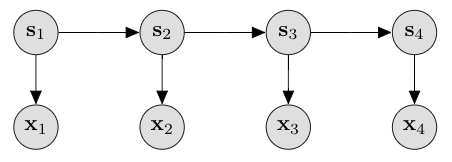
\includegraphics{hmm_p2}
	\end{center}
	(all nodes are observed)
	
	\item $N=1$, the number of sequences observed\\
	$n=4$, the length of the sequences\\
	$c=2$, the number of states a hidden state can take\\
	$\bolds^1_1 = [1 \ 0]^\top, \bolds^1_2 = [0 \ 1]^\top, \bolds^1_3 = [0 \ 1]^\top, \bolds^1_4 = [1 \ 0]^\top$\\
	$\boldx^1_1 = [1 \ 0]^\top, \boldx^1_2 = [0 \ 1]^\top, \boldx^1_3 = [0 \ 1]^\top, \boldx^1_4 = [0 \ 1]^\top$
	\item $\hat{\boldsymbol{\theta}} = [1 \ 0]^\top$, the distribution of the weather for the initial state\\
	$\hat{\boldT} = \begin{bmatrix} 0 & 1 \\ \frac{1}{2} & \frac{1}{2} \end{bmatrix}$, the transition probabilities for the weather\\
	$\hat{\boldsymbol{\pi}}_1 = [\frac{1}{2} \ \frac{1}{2}]^\top$, the distribution of cloud colors on sunny days\\
	$\hat{\boldsymbol{\pi}}_2 = [0 \ 1]^\top$, the distribution of cloud colors on rainy days
\end{enumerate}
\end{solution}

\newpage
\fbox{\parbox{\linewidth}{%
		\textbf{EM for HMMs.} You are trying modeling a toy's state using an HMM. At each time step, the toy can be active (state 1) or inactive (state 2), but you can only observe the color of the indicator light, which can be red (observation state 1) or green (observation state 2). You have collected data from one sequence:\\
		\centerline{
			\begin{tabular}{c|c}
				\text{Time} & \text{Light}\\\hline
				1 & \text{Green}\\
				2 & \text{Red}\\
				3 & \text{Green}
		\end{tabular}}
		You initialize your EM with $\boldsymbol{\theta} = [\frac{1}{2} \ \frac{1}{2}]^\top, \boldT = \begin{bmatrix} \frac{2}{3} & \frac{1}{3} \\ \frac{1}{3} & \frac{2}{3} \end{bmatrix}, \boldsymbol{\pi}_1 = [\frac{1}{4} \ \frac{3}{4}]^\top, \boldsymbol{\pi}_2 = [\frac{3}{4} \ \frac{1}{4}]^\top$.
		\begin{enumerate}
			\item Compute $\alpha_1, \alpha_2, \alpha_3, \beta_1, \beta_2, \beta_3$ for the forward-backward algorithm using the initial parameter values.
			\item How is $\boldq^1_{t}$ defined? Compute the values of $\boldq^1_1, \boldq^1_2$ using the $\alpha$ and $\beta$ values.
			\item How is $\boldQ^1_{t,t+1}$ defined? Compute the value of $\boldQ^1_{1,2}$ using the $\alpha$ and $\beta$ values.
		\end{enumerate}
		\vspace{0.2cm}
		During EM, at one point you obtain the following values after the E step:
		\[ \boldq^1_1 = \left[ \frac{2}{3} \ \frac{1}{3} \right]^\top, \quad \boldq^1_2 = \left[ \frac{1}{3} \ \frac{2}{3} \right]^\top, \quad \boldq^1_3 = \left[ \frac{2}{3} \ \frac{1}{3} \right]^\top\]
		\[\boldQ^1_{1,2} = \begin{bmatrix} \frac{1}{6} & \frac{1}{2} \\ \frac{1}{6} & \frac{1}{6} \end{bmatrix}, \quad \boldQ^1_{2,3} = \begin{bmatrix} \frac{1}{6} & \frac{1}{6} \\ \frac{1}{2} & \frac{1}{6} \end{bmatrix} \]
		\begin{enumerate}
			\setcounter{enumii}{3}
			\item Use the above values to compute $\hat{N}_k, \hat{N}_{kl}, \hat{N}_{kj}$.
			\item Complete the M step by updating the parameters $\boldsymbol{\theta}, \boldT, \boldsymbol{\pi}_1, \boldsymbol{\pi}_2$.
		\end{enumerate}
}}

\begin{solution}
\begin{enumerate}
	\item Using the recursive defintions for $\alpha, \beta$ and the current values of $\boldsymbol{\theta}, \boldT, \boldsymbol{\pi}_1, \boldsymbol{\pi}_2$:
	\def\arraystretch{1.5}
	\begin{align*}
	\alpha_1(\bolds^1_1) &= \left\{
	\begin{array}{ll}
	\frac{3}{8} & \bolds^1_1 = \text{active} \\
	\frac{1}{8} & \bolds^1_1 = \text{inactive}
	\end{array} 
	\right.\\
	\alpha_2(\bolds^1_2) &= \left\{
	\begin{array}{ll}
	\frac{7}{96} & \bolds^1_2 = \text{active} \\
	\frac{15}{96} & \bolds^1_2 = \text{inactive}
	\end{array} 
	\right.\\
	\alpha_3(\bolds^1_3) &= \left\{
	\begin{array}{ll}
	\frac{29}{384} & \bolds^1_3 = \text{active} \\
	\frac{37}{1152} & \bolds^1_3 = \text{inactive}
	\end{array} 
	\right.\\
	\beta_3(\bolds^1_3) &= \left\{
	\begin{array}{ll}
	1 & \bolds^1_3 = \text{active} \\
	1 & \bolds^1_3 = \text{inactive}
	\end{array} 
	\right.\\
	\beta_2(\bolds^1_2) &= \left\{
	\begin{array}{ll}
	\frac{7}{12} & \bolds^1_2 = \text{active} \\
	\frac{5}{12} & \bolds^1_2 = \text{inactive}
	\end{array} 
	\right.\\
	\beta_1(\bolds^1_1) &= \left\{
	\begin{array}{ll}
	\frac{29}{144} & \bolds^1_1 = \text{active} \\
	\frac{37}{144} & \bolds^1_1 = \text{inactive}
	\end{array} 
	\right.
	\end{align*}
	\item $q^1_{tk}$ is the probability that $\bolds^1_t$ is $S_k$ (given the observations), and $q^1_{tk} = p(\bolds^1_t = S_k \mid \boldx^1; \boldw) \propto \alpha_t(S_k) \beta_t(S_k)$. Then $\boldq^1_1 \propto [\frac{87}{1152} \ \frac{37}{1152}]^\top$, so $\boldq^1_1 = [\frac{87}{124} \ \frac{37}{124}]^\top$. Also, $\boldq^1_2 \propto [\frac{49}{1152} \ \frac{75}{1152}]^\top$, so $\boldq^1_2 = [\frac{49}{124} \ \frac{75}{124}]^\top$.
	\item $q^1_{t,t+1,k,l}$ is the probability that $\bolds^1_t$ is $S_k$ and $\bolds^1_{t+1}$ is $S_l$ (given the observations), and $q^1_{t,t+1,k,l} = p(\bolds^1_t = S_k, \bolds^1_{t+1} = S_l \mid \boldx^1; \boldw) \propto \alpha_t(\bolds_t) p(\bolds_{t+1} \mid \bolds_t) p(\boldx_{t+1} \mid \bolds_{t+1}) \beta_{t+1}(\bolds_{t+1})$. Then 
	\[\boldQ^1_{1,2} \propto \begin{bmatrix} \frac{42}{1152} & \frac{45}{1152} \\ \frac{7}{1152} & \frac{30}{1152} \end{bmatrix}\]
	so 
	\[\boldQ^1_{1,2} = \begin{bmatrix} \frac{42}{124} & \frac{45}{124} \\ \frac{7}{124} & \frac{30}{124} \end{bmatrix}\]
	\item 
	\begin{align*}
	\text{For $\hat{N}_k$:}& \quad \hat{N}_1 = \frac{5}{3}, \quad \hat{N}_2 = \frac{4}{3}\\
	\text{For $\hat{N}_{kl}$:}& \quad \hat{N}_{1,1} = \frac{1}{3}, \quad \hat{N}_{1,2} = \frac{2}{3}, \quad \hat{N}_{2,1} = \frac{2}{3}, \quad \hat{N}_{2,2} = \frac{1}{3}\\
	\text{For $\hat{N}_{kj}$:}& \quad \hat{N}_{1,1} = \frac{1}{3}, \quad \hat{N}_{1,2} = \frac{4}{3}, \quad \hat{N}_{2,1} = \frac{2}{3}, \quad \hat{N}_{2,2} = \frac{2}{3}
	\end{align*}
	\item
	$\boldsymbol{\theta} = [\frac{2}{3} \frac{1}{3}]^\top$\\
	$\boldT = \begin{bmatrix} \frac{1}{3} & \frac{2}{3} \\ \frac{2}{3} & \frac{1}{3} \end{bmatrix}$\\
	$\boldsymbol{\pi}_1 = [\frac{1}{5} \frac{4}{5}]^\top$\\
	$\boldsymbol{\pi}_2 = [\frac{1}{2} \frac{1}{2}]^\top$
	
\end{enumerate}
\end{solution}

\end{document}
